\newcommand{\Release}{}% Set Release or other word
\newcommand{\Slide}{}% Rename other than 'Slide' to make A4
\newcommand{\PrintLecture}{1}% Lecture On(1)/Off(0)
\newcommand{\PrintSolution}{1}% Solution(Answer) On(1)/Off(0)
\newcommand{\MyCourse}{データサイエンスコース}
\newcommand{\MySemester}{春}
\newcommand{\MySubject}{ビジネス アナリティクス}
\newcommand{\MyClass}{第17回ー分類}% フォルダ名自動挿入

%
% 科目共通定義
%

\newcommand{\OpenIntro}
{\MyRef{OpenIntro Statistics}{https://www.openintro.org/book/os}}

\newcommand{\R}{\textbf{R}}
\newcommand{\RStudio}{\textbf{RStudio}}
\newcommand{\Excel}{\textbf{Excel}}
\newcommand{\cs}[1]{\textcolor{blue}{\texttt{#1}}} % Console prompt >

\newcommand{\ra}{\rightarrow}
\newcommand{\Ra}{\Rightarrow}

% Expectation E[X]
\def\E#1{E\big[#1\big]}
\def\S{\sum_{i=1}^n}

\newcommand{\B}{\hat{\beta}}
\newcommand{\SUM}{\sum_{i=1}^n}  % Summention from i=1 to n
\newcommand{\NH}{$\mathit{H}_0$} % Null hypthesis
\newcommand{\AH}{$\mathit{H}_1$} % Alternative hypothesis
\newcommand{\T}{\texorpdfstring{$t$}{}}% Student's t
\newcommand{\overtext}[3][1.5]{
  \mathrel{\overset{#2}{\scalebox{#1}[1]{$#3$}}}
}
\newcommand{\iid}{\overtext[2]{iid}{\sim}}
\newcommand{\convdist}{\overtext[2]{d}{\rightarrow}}
\newcommand{\convprob}{\overtext[2]{p}{\rightarrow}}
\newcommand{\as}[2]{\quad \text{as}\quad #1 \rightarrow #2}

\input{../../tex/hss_lualatex.tex}
\input{../../tex/hss_moodle.tex}
\input{../../tex/hss_beamer.tex}

\begin{document}

\section{小テスト(\MyClass)}

\begin{quiz}{\MyClass}

\QuizShortAnswer
{
  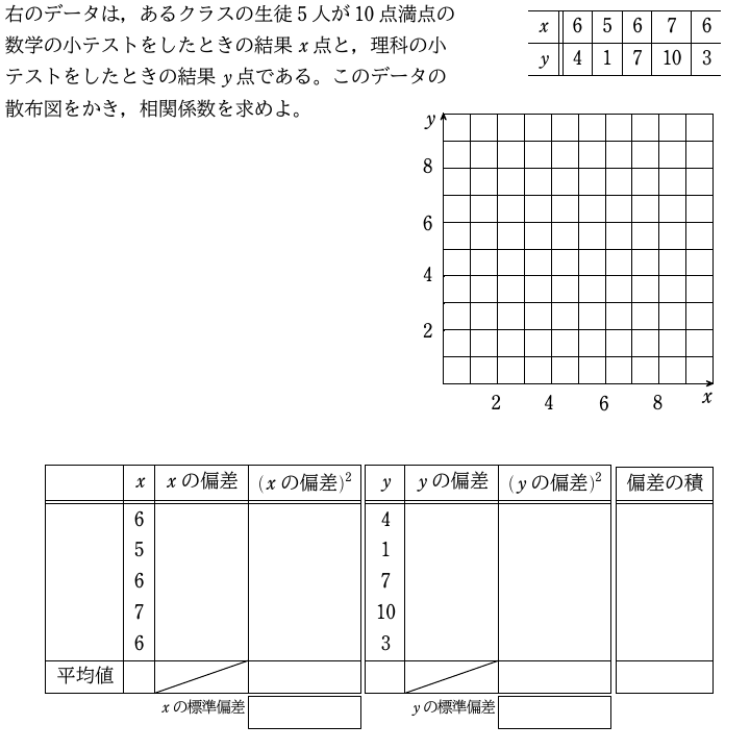
\includegraphics[width=0.6\textwidth]{quiz/problem53.png}\\
  解答欄には相関係数の値を記入すること.
}
{
  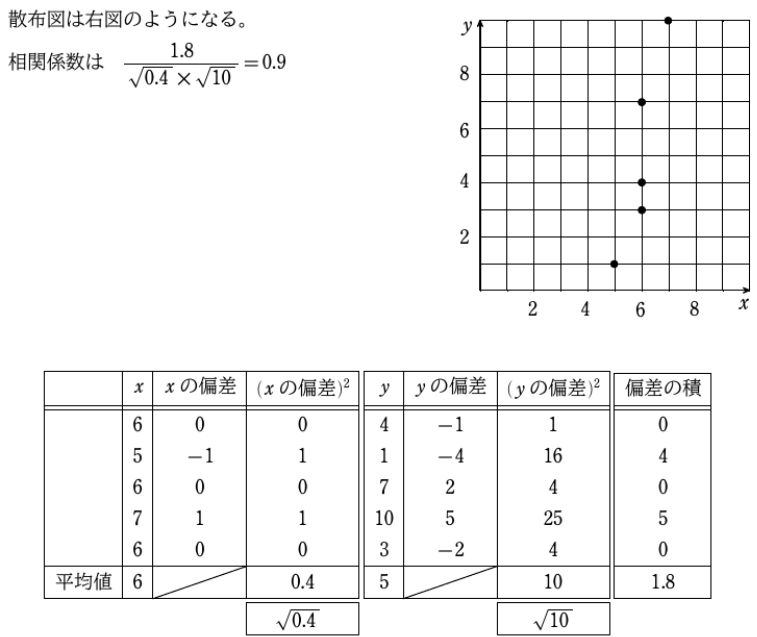
\includegraphics[width=0.6\textwidth]{quiz/solution53.png}
}
{100}
{0.9}
{}
{}
{}

\end{quiz}

\end{document}
